%%%%%%%%%%%%%%%%%%%%%%%%%%%%%%%%%%%%%%%%%%%%%%%%%%%%%%%%%%%%%%%%%%%%%%%%

%%% LaTeX Template for AAMAS-2023 (based on sample-sigconf.tex)
%%% Prepared by the AAMAS-2023 Program Chairs based on the version from AAMAS-2022. 

%%%%%%%%%%%%%%%%%%%%%%%%%%%%%%%%%%%%%%%%%%%%%%%%%%%%%%%%%%%%%%%%%%%%%%%%

%%% Start your document with the \documentclass command.
%%% Use the first variant below for the final paper.
%%% Use the second variant below for submission.

%\documentclass[sigconf]{aamas} 
\documentclass[sigconf,anonymous]{aamas} 

%%% Load required packages here (note that many are included already).
\newcommand{\set}[1]{\{#1\}}
\usepackage{balance} % for balancing columns on the final page
\usepackage{dsfont}

%%%%%%%%%%%%%%%%%%%%%%%%%%%%%%%%%%%%%%%%%%%%%%%%%%%%%%%%%%%%%%%%%%%%%%%%

%%% AAMAS-2023 copyright block (do not change!)

\setcopyright{ifaamas}
\acmConference[AAMAS '23]{Proc.\@ of the 22nd International Conference
on Autonomous Agents and Multiagent Systems (AAMAS 2023)}{May 29 -- June 2, 2023}
{London, United Kingdom}{A.~Ricci, W.~Yeoh, N.~Agmon, B.~An (eds.)}
\copyrightyear{2023}
\acmYear{2023}
\acmDOI{}
\acmPrice{}
\acmISBN{}

%%%%%%%%%%%%%%%%%%%%%%%%%%%%%%%%%%%%%%%%%%%%%%%%%%%%%%%%%%%%%%%%%%%%%%%%

%%% Use this command to specify your EasyChair submission number.
%%% In anonymous mode, it will be printed on the first page.

\acmSubmissionID{???}

%%% Use this command to specify the title of your paper.

\title[AAMAS-2023 Formatting Instructions]{Source Detection in Networks using the Stationary Distribution of a Markov Chain}

%%% Provide names, affiliations, and email addresses for all authors.

\author{Yael Sabato}
\affiliation{
  \institution{Computer Science Department }
  \city{Ariel University}
  \country{Israel}}
\email{yael.sabato@msmail.ariel.ac.il}

\author{Amos Azaria}
\affiliation{
  \institution{Data Science Center, Computer Science Department}
  \city{Ariel University}
  \country{Israel}}
\email{amos.azaria@ariel.ac.il}

\author{Noam Hazon}
\affiliation{
  \institution{Computer Science Department}
  \city{Ariel University}
  \country{Israel}}
\email{noamh@ariel.ac.il}

%%% Use this environment to specify a short abstract for your paper.

\begin{abstract}
Nowadays, the diffusion of information or infection through social networks is a common and a powerful phenomenon. One common way to model diffusions in social networks is the Independent Cascade (IC) model. %, which is a stochastic.
Given a set of infected nodes according to the IC model, a natural problem is the source detection problem, in which the goal is to identify the unique node that has started the diffusion.
Maximum Likelihood Estimation (MLE) is a common approach for tackling the source detection problem, but it is computationally hard.

In this work, we propose an efficient method for the source detection problem under the MLE approach, which is based on computing the stationary distribution of a Markov chain. Using simulations, we demonstrate the effectiveness of our method compared to other state-of-the-art methods from the literature.

\end{abstract}

%%% The code below was generated by the tool at http://dl.acm.org/ccs.cfm.
%%% Please replace this example with code appropriate for your own paper.


%%% Use this command to specify a few keywords describing your work.
%%% Keywords should be separated by commas.

\keywords{Source detection, Maximum likelihood, Markov chain}

%%%%%%%%%%%%%%%%%%%%%%%%%%%%%%%%%%%%%%%%%%%%%%%%%%%%%%%%%%%%%%%%%%%%%%%%

%%% Include any author-defined commands here.
         
\newcommand{\BibTeX}{\rm B\kern-.05em{\sc i\kern-.025em b}\kern-.08em\TeX}

%%%%%%%%%%%%%%%%%%%%%%%%%%%%%%%%%%%%%%%%%%%%%%%%%%%%%%%%%%%%%%%%%%%%%%%%

\begin{document}

%%% The following commands remove the headers in your paper. For final 
%%% papers, these will be inserted during the pagination process.

\pagestyle{fancy}
\fancyhead{}

%%% The next command prints the information defined in the preamble.

\maketitle 

%%%%%%%%%%%%%%%%%%%%%%%%%%%%%%%%%%%%%%%%%%%%%%%%%%%%%%%%%%%%%%%%%%%%%%%%

\section{Introduction}

%and related work
%There are many cases of spreads in networks
Nowadays, the diffusion of information or infection through social networks is a common %an interesting 
and a powerful phenomena. In this work, our goal is, given a set of active or infected nodes, to seek the unique node that started the diffusion.

%Many approaches, most do not assume knowledge of the probabilities
There are many approaches to this computational problem in the literature, each assuming different spreading models and various amounts of knowledge of the network parameters. In general, most of the  approaches do not assume full information of the diffusion probabilities. In our work we assume the diffusion matches the independent cascade model, and we have full information on the diffusion probabilities of the social network.
%If we have the probabilities, we should use MLE
Assuming we have complete knowledge of those parameters, the mathematical approach should be computing a parameter of likelihood to each node, and output the node with the maximum likelihood.
%Some assume: Effector problem, but did not use MLE

%MCMC use MLE, but they are slow

%We propose fast and accurate MLE
In this work we study the problem of finding the source of a diffusion in the Independent cascade model, and we assume we have full information of the diffusion parameters of the users in the social network.
We propose an efficient method for this problem. Our method utilizes the maximum likelihood approach and is based on computing the stationary distribution of a Markov chain.
%In order to find the most likely source, we use an evaluation of the number of possible spreading patterns for each node. %(to add - each spreading pattern has it's probability)
%%%%%%%%%%%%%%%%%%%%%%%%%%%%%%%%%%%%%%%%%%%%%%%%%%%%%%%%%%%%%%%%%%%%%%%%

\section{Related Work}

% 1. source detection in general
% various models SI, SIR, IC
% various amount of information of the graph parameters
% 2. our approach to source detection  


%11/11: 
Viral spread of information trough social networks, inspired various research. The Influence Maximization problem is to find the (prior) most influential node (or set of nodes) in a social network. another interesting problem is, finding the source of a spread that already happened. In a way, it is like finding the most influential node of a given subset of the graph %...


The first paper to formalize the computational problem of finding the source of a diffusion in a network, were \cite{lappas2010finding} (and \cite{shah2010detecting}).  \cite{lappas2010finding} formalized this computational problem, where given a set of active nodes, that are a result of a diffusion of the Independent cascade model, they seek the set of $k$ nodes that best explain the given activation set. \cite{lappas2010finding} did not use the Maximum Likelihood Estimation approach (Many papers already pointed that out).



%other works assumed very little graph information and studied various methods to estimate the graph parameters.

%we wanted to see how accurate we can be if we have full information on the graph parameters.... 

Most of the research of this problem was: to find an algorithm for finding the source on a restricted type of graphs, (a directed tree, or a DAG), and then for general graphs, to take (once or more, randomly or not) subgraphs of the original (general) graph that matches the type in question, and apply the first algorithm to obtain grades to each node. Finally, the output is the node with the highest sum of grades.

the approach of the Markov tree theorem is to take in account all the possible spread patterns at once.


%A few sentences on each paper that we concentrate on:
\cite{lappas2010finding}
Lappas at al. was the first to formulate the source detection computational problem. They considered the Independent cascade model of diffusion. but did not use a Maximum likelihood approach


\cite{shah2010detecting}
considered the SIR model, 
Their algorithm is based on rumor centrality. they basically calculate it on trees. and when getting back to a general graph, they concentrate only on a BFS tree (coming out of each node)

\cite{shah2011rumors}
SI model, rumor centrality vs distance centrality
BFS trees.

\cite{zhai2015cascade}
IC model
they prove $sharp$ p-completeness %(#p)
they use the concept of Markov chain in order to sample sub graphs of the social network. here the states of the Markov chain that they built are different samples of the social graph. for each such sample they calculate the set of all possible source nodes (I.e. nodes that can reach each of the active nodes with a positive probability path. we later call this set $A'$.)

their algorithm is to conduct a random walk on the above Markov chain, and for every sample to increase the grades of all the nodes of A', they do $10^6$ iterations and output the node with the maximum grade.

(They used the graph wiki-vote...)

\cite{zhang2017markov}
a similar idea of the above MCMC, but with the Linear Treshold model....

\cite{kumar2017temporally} 
They consider SI model, but then they say that their algorithm is agnostic of the underline diffusion model.
they used the Markov chain tree theorem for evaluating the most likely source. but assumed that each node is equally likely to get activated from each of it's neighbours. (also, they consider varying present of given activating edges...)

reviews: \cite{shelke2019source}, \cite{jiang2016identifying}, \cite{jin2021schemes}

\cite{zhu2015source} also is dealing with the problem of finding the most likely sub tree. their algorithm is called SFT (for "short-fat-trees")

\cite{farajtabar2015back} partially observed cascade. the information on the active set is partial. their algorithm includes finding the most likely graph and also finding the source node.
they use CTIC continuous time independent cascade madel.

\cite{tong2016effector}
they show an algorithm on DAG's and for general graphs they extract a sub graph of the social network that is a DAG and then apply their algorithm.
(They want to find the sub DAG that has the maximum entropy, but it is NP-hard, so they have a permutation based heuristic to extract the DAG)
%I'm not sure we should add this one, but it is interesting:
\cite{gomez2012inferring} (and Jure Leskovec)
their input are diffusions, they try to learn the graph that best explain the given diffusion. 


Our contribution:
1. we developed the approach of \cite{kumar2017temporally} to a model where there are various edge probabilities. we show how to normalize the edge probabilities in order to get a valid Markov chain.
%(maybe to add, here or later:) In addition, we divide our algorithm to 2 stages, and give information on the amount of times the algorithm returned the right answer in the first (trivial) stage.
% Indeed, their approach for calculating the occurrence probability is based on a simple multiplications of the e for each out-tree the probability that of all its edges appear, and ignore all the other edges of the graph. resulting with an inclusion exclusion problem. (as mentioned in the previous section.)


They also assume that the graph is undirected, so they show a method for converting the undirected social graph into an irreducible Markov Chain, by replacing each undirected edge ${u,v}$ by two directed edges $(u,v)$ and $(v,u)$.
(they also assume that a fraction of the activating edges are given as input. and that the underline diffusion model is a SI model. but they say that since thay are consentrait in spreading paterns, they can be agnostic of the )
%(so maiffybeusion mod this el.isprecise d our work, of matching their framework to the IC model.)


%%%%%%%%%%%%%%%%%%%%%%%%%%%%%%%%%%%%%%%%%%%%%%%%%%%%%%%%%%%%%%%%%%%%%%%%

\section {Preliminaries}
\subsection{Directed Rooted Trees}
A directed rooted tree is a directed acyclic graph (DAG) whose underlying undirected graph is a tree, and one of its vertices has been designated the root.
An out-tree is a directed rooted tree, in which all the edges point away from the root. Similarly, an in-tree is a directed rooted tree, in which all the edges point toward the root. Clearly, we can convert an out-tree into an in-tree by reversing the directions of the edges. A spanning in-tree/out-tree is an in-tree/out-tree that spans all vertices of the underlying graph. 
%(!! not connected to in/out-trees,AND we say something similar in the next section:) We denote by $d_{in}(v)$ the in-degree of a node $v$.
\subsection{The Diffusion Model}
\label{sec:IC_model}
The research on the diffusion of information on social networks has considered several models. In this paper we focus on the independent cascade model (IC), which is the following.
There is a social network that is represented by a weighted directed graph $G_N=(V_N,E_N)$ with no self loops, where each user of the social network is represented by a node, every connection between two users is an edge, and the weights represent the influence probabilities. 
The process of diffusion concerns a message that is propagated thorough the social network. During this process, each node can either be inactive or become active.
The diffusion process starts with an initial source   
$v\in V_N$, which is the first active node.
The process then unfolds in discrete steps according to the following rule. %If a node $v$ was inactive in step $t-1$ and became active in step $t$, 
Every node $v_i\in V_N$ that becomes active in step $t-1$, attempts to activate each currently inactive neighbor $v_j$ in step $t$, and only in step $t$. The probability that $v_i$ succeeds in activating an inactive neighbor $v_j$ is $p^{ij}$, which is the weight of the edge $(v_i,v_j)\in E_N$. We denote by $w_{in}(v_i)$ the weighted in-degree of a node $v_i$, $w_{in}(v_i) = \sum_j{p^{ji}}$.
%, independently of the history until this time. 
If multiple neighbors of a vertex $v$ try to activate it at the same time, their attempts are considered in an arbitrary order. %$v$ does not attempt to activate its neighbors again. 
The process runs until no more activations occur. %are possible.

Note that since each active node is activated by a single parent, the active nodes and activating edges %(!! do we need to define an "activating edge"?) 
form an out-tree, which spans the set of active nodes, and the source node is the root of the tree.

%As shown by \citeauthor{kempe2003maximizing} \cite{kempe2003maximizing}, the diffusion process is equivalent to first selecting the participating edges according to their probabilities, (by a series of coin flips with the corresponding probability) obtaining a graph of connections $G'=(V,E')$. Then, every node $v \in V$ of the graph that has a directed path starting from one of the nodes of the source and ending at $v$ is assumed to be active.
%We note that in $G'$ all edges, $E'$, have a fixed probability of $1.0$.


\subsection{Markov Chain}
\label{sec:maarkov_chain}


A (discrete-time) Markov chain is %a stochastic model that contains 
an infinite sequence of discrete random variables $(X_i)_{i=0}^{\infty}$.
All variables have the same finite set of possible values, $S = \set{s_1,s_2,\ldots,s_k}$, which is called the state set of the Markov chain.
The variables of the sequence $(X_i)_{i=0}^{\infty}$ have the Markov property of \textit{forgetfulness}, that is, each variable $X_t$ is dependent only on the previous variable $X_{t-1}$, and is independent of all other previous variables. Moreover, all the variables have the same probability distribution.
Namely, for every $t>0$, $P(X_{t}=s_{i_t}|X_1=s_{i_1},X_2=s_{i_2},...,X_{t-1}=s_{i_{t-1}}) =P(X_{t}=s_{i_t}|X_{t-1}=s_{i_{t-1}})=P(X_{t+1}=s_{i_t}|X_{t}=s_{i_{t-1}})$, where $s_{i_j} \in S$. For a pair of states $s_i$ and $s_j$, let $q^{ij}=P(X_{t}=s_j|X_{t-1}=s_i)$. We call $q^{ij}$ the \textit{transition probability}. Note that $\sum_{j=1}^k{q^{ij}}=1$. 

%(!! I think we don't need this:) 
%The \textit{n-step transition probability} is $q^{ij}_{(n)}=P(X_{t}=s_j|X_{t-n}=s_i)$.

%the probability that a process in state $s_j$ will be in state $s_i$ after $n$ additional transitions.

A Markov chain can be represented as a weighted directed graph $G_M=(S_M,E_M)$, where each state is represented by a node. For clarity reasons, we refer to the nodes of $S_M$ as states.
There is an edge $(s_i,s_j) \in E_M$ if the transition probability $q^{ij}>0$, with a weight of $q^{ij}$.
%Note that for each state $s \in V_M$, the sum of the weights of its out edges equals $1$.
A random walk on the graph $G_M$ is called a Markov process.

\subsubsection{Irreducibility}
A Markov chain is \textit{irreducible} if for each pair of states $s_i,s_j$, there are two directed paths $s_i \leadsto
s_j$ and  $s_j \leadsto
s_i$ in $G_M$. That is, a Markov chain is irreducible if its graph, $G_M$, is strongly connected.

\subsubsection{Stationary Distribution}

If the Markov chain is irreducible
then the long run average number of visits
of the Markov process to any state $s_i$, converges to a number $\Pi_i$, 
regardless of the initial state. That is, for all 
$s_i\in S$ it holds that 
%
$\Pi_i = \lim_{n\rightarrow \infty}\frac{1}{n}\sum_{t=0}^{n-1} \mathbb{I}(X_t=s_i)$, 
%
%
where $\mathbb{I}(\cdot)$ is an indicator function. Moreover, $\Pi = (\Pi_1,$ $\Pi_2,$ $\ldots,$ $\Pi_n)$ is a probability distribution over the set of states $S$, which is called the \textit{Stationary Distribution}\footnote{Some works provide a slightly different definition for the stationary distribution, which requires that the Markov chain will also be ergodic \cite{batabyal2006markov}.}.
The stationary distribution can be computed in polynomial time using the  %\cite{??}.
However, if $G_M$ is very large the exact computation of the stationary distribution may become impractical; in this case, it is common to estimate the stationary distribution by sampling, i.e., using random walks on the graph % what do you think about this cite? is it good? \cite{levin2017markov}.
%(!!)

\subsection{Vector Notations}

Let $V$ be a vector, $V= (V_1, V_2, \ldots ,V_n)$. We denote by $\hat{V}$ the normalized vector, $\hat{V} = (\frac{V_1}{\sum_{i=1}^n V_i}, \frac{V_2}{\sum_{i=1}^n V_i}, \ldots ,\frac{V_n}{\sum_{i=1}^n V_i})$.

%%%%%%%%%%%%%%%%%%%%%%%%%%%%%%%%%%%%%%%%%%%%%%%%%%%%%%%%%%%%%%%%%%%%%%%%%%%%%%%%%%%%%%%%%%%%%%%%%%%%%%%%%%5


\section{Problem Statement} \label{sec: problem statement} 
In this section, we define the source detection problem and present the MLE principle, which provides a framework for addressing it.
%problem definition
\begin{definition}[Source Detection]
Given a social network, $G_N=(V_N,E_N)$, and a set of active nodes $A\subseteq V_N$ at the end of a propagation process that is compatible to the IC diffusion model, find the source node. 
\end{definition}

We first note that a source node $v$ must be in $A$. Moreover, there must be a directed path from $v$ to each node in $A$. %i.e., there is an out-tree from $v$ that spans all the nodes of $A$. 
Let $A' \subseteq A$ be the set of all nodes that have directed paths to all nodes in $A$. Clearly, $A'$ is strongly connected.
In addition, if $A'$ is the singleton $\set{v}$ then $v$ is the source node.

%our approach - MLE: evaluate which node is the most likely
Our approach for identifying the source node is to follow the maximum likelihood principle \cite{myung2003tutorial}. That is, each node is associated with the probability that it is the source, and we select a node with the maximal probability. Formally, let $R_i$ be the event that $v_i$ is the source node, and let $\mathcal{A}$ be the event that the set $A$ is the set of active nodes; $\mathcal{A'}$ is defined similarly for $A'$. We would like to solve the following problem:

\begin{definition}[ML-Source]
Given a social network, $G_N=(V_N,E_N)$, and a set of active nodes $A\subseteq V_N$ at the end of a propagation process according to the IC diffusion model, find the most likely source node $v^*$, i.e.,\\ $
v^* = \arg\max_{v_i \in V_N} P(R_i | \mathcal{A}).
$ 
\end{definition}
\noindent Note that $P(R_i | \mathcal{A}) = \frac{P(R_i,\mathcal{A})}{P(\mathcal{A})}$, and thus 
$$
\arg\max_{v_i \in V_N} P(R_i | \mathcal{A}) = \arg\max_{v_i \in V_N} P(R_i,\mathcal{A}).$$
%
%For each active node $v\in A$, we call the node that activated it, $v$'s \textit{activator}, and we call the edge between $v$'s activator and $v$, an \textit{activating edge}.

Unfortunately, the ML-Source problem was shown to be computationally hard~\cite{zhai2015cascade}.
Indeed, the following brute-force procedure computes the exact value of $P(R_i,\mathcal{A})$, in exponential time.
%We first compute the set $A'$ using BFS from each node $v \in A$ (if $|A'|=1$, we can stop) %(!!or return...). 
Let $G_N[A] = (A, E(A))$ be the subgraph of $G_N$ induced by the set $A$. That is, $E(A)$ is the set of edges of $G_N$ that have both nodes in $A$.
We consider every subset $X\subseteq E(A)$, and each such $X$ is associated with a probability for its occurrence: 
$$
p(X)=\prod_{e\in X}p^e\cdot \prod_{e\in E(A)\setminus X} (1-p^e).
$$
Let $G_X$ be a graph, $G_X =(A,X)$. If there exists an out-tree in $G_X$ that spans $A$ and with the node $v_i$ as the root, then the probability $p(X)$ should be added to $P(R_i,\mathcal{A})$. Namely:
$$
P(R_i,\mathcal{A}) = \sum_{X\subseteq E(A)} I (X,v_i)\cdot p(X)
$$
where $I(X,v_i)$ is an indicator function that returns $1$ if the graph $G_X$ has a spanning out-tree with $v_i$ as the root, and $0$ otherwise.
In order to return the most likely source node, one should compute the above expression for every $v_i\in A$. Moreover, each $p(X)$ can be used more than once, in the case where $G_X$ has multiple spanning out-trees with several roots.

\section{The Markov Chain Approach}
\citeauthor{kumar2017temporally}~\cite{kumar2017temporally} suggested the Markov chain approach for estimating the probability of a node to be the source, in their setting.
%$P(R_i,\mathcal{A})$. 
Their main idea is to count for each node $v$ every possible spanning out-tree, in which $v$ is the root, and for each such out-tree to calculate its occurrence probability. 

We adapt the Markov chain approach to our setting, as follows.

For a diffusion that started with a source node $v_i$, and
resulted with a set $A$ of active nodes,  
let $T_{i,A}$ be the corresponding spanning out-tree, and let $\mathcal{T}_{i,A}$ be the associated event. We denote by $w(T)$ the weight of a directed rooted tree, $w(T) = \prod_{e\in T}p^e$.
A good estimation of the probability of $\mathcal{T}_{i,A}$ is:
$$
P(\mathcal{T}_{i,A}) \approx P(R_i)\cdot w(T_{i,A}).
$$
Note that this is an estimation, since we ignore the edges that are not part of the spanning out-tree. % (even though they may happen to be activating edges).
In order to calculate the probability of a single node $v_i$ to be the source, we go over every spanning out-tree rooted at $v_i$ and sum the weights of those out-trees:

%$P(R_i,\mathcal{A})$ by:
$$
P(R_i,\mathcal{A}) \approx \sum _{T_{i,A}\in OT_{i,A}} P(\mathcal{T}_{i,A}).
$$
where $OT_{i,A}$ is a set of all the out-trees of $G_N[A]$ that are rooted at $v_i$ and span $A$. 
Note that this summation is also an estimation, since the events $\mathcal{T}_{i,A}$ for every spanning out-tree are not independent (which can be fixed with an inclusion-exclusion calculation).


%In addition, for each node $v_i\in V_N$ let $H_{i,A}$ be the set of all out-trees rooted at $v_i$ that span $A$.
%Then, % a good estimation for $P(R_i,\mathcal{A})$ is:
%we can estimate %compute 


For  $v_i \in A'$, let $\Gamma_i =  \sum _{T_{i,A'}\in OT_{i,A'}} w(T_{i,A'})$, let $\Gamma =(\Gamma_1,$ $ \Gamma_2,$ $\ldots,$ 
$\Gamma_{|A'|})$, 
and let $\hat{\Gamma} =
\frac{1}{\sum_{i=1}^{|A'|}\Gamma_i}\cdot 
(\Gamma_1,$ $ \Gamma_2,$ $\ldots,$ $\Gamma_{|A'|})$  
% nov 22 alternatively:
% and let $\Gamma$ be a vector where every $\Gamma_i$ is places in the $i$'th position
We assume that the \textit{prior} probability, $P(R_i)$, is equal for every $v_i\in V_N$. It is also enough to consider $A'$ instead of $A$ since $P(R_i,\mathcal{A}) \propto P(R_i,\mathcal{A'})$ (according to \cite{kumar2017temporally}). 
We get that
\begin{equation}
\label{eq: v* by spreading patterns}    
v^* \approx \arg\max_{v_i \in A'} \Gamma_i.
\end{equation}

Based on this formulation, a naive approach is to compute for each $v_i\in A'$ the set $OT_{i,A'}$, (using an algorithm for finding all spanning out-trees, e.g. \cite{gabow1978finding}), and to return the node $v_i$ that maximizes $\Gamma_i$. We refer to this approach as the out-tree counting method.
Clearly, the out-tree counting method is (also) computationally expensive, as the size of $OT_{i,A'}$ is most likely exponential in $|A'|$. 
We thus propose to use the following theorem 
\cite{leighton1986estimating}:

Given a finite state irreducible Markov chain as a directed graph $G_M=(S_M,E_M)$, 
Let $w(T) = \prod_{e\in T} p^e$ be the weight of a spanning in-tree $T \subseteq E_M$. Let $IT_{i,S_M}$ be the set of all in-trees in $E_M$ that have $s_i$ as their root and span $S_M$. Let $\Psi_i:= \sum _{T\in IT_{i,S_M}}w(T)$, let $\Psi = (\Psi_1, \Psi_2, \ldots, \Psi_n)$, and let $\hat{\Psi} =\frac{1}{\sum_{i=1}^{n}\psi_i}\cdot (\Psi_1, \Psi_2, \ldots, \Psi_n)$.

\begin{theorem} \label{TreeThm}
(Markov chain tree theorem)
Given a finite state irreducible Markov chain, For every $s_i\in S_M$, the unique Stationary Distribution $\Pi_i$ equals to $\hat{\Psi}_i$:
\begin{equation}
\forall s_i\in S_M,  \Pi_i = \hat{\Psi}_i = \frac{\Psi_i}{\sum _{j=1}^n\Psi_j}    
\end{equation}
\end{theorem}

%Let $G_N[A']$ be the subgraph of $G_N$ induced by the set $A'$.
%8/9/22 addition:
%In addition, we call $\Gamma_i$ the expression we use as our heuristic, $\Gamma_i =  \sum _{T_{i,A'}\in OT_{i,A'}} w(T_{i,A'})$.
Our approach is based on exploiting the structural similarity between $\Gamma$ and $\Psi$. Indeed, let $G_N[A']$ be the graph $G_N$ induced on the set $A'$, then for every $1\leq i\leq |A'|$, $\Gamma_i$ is the summation of weights of spanning out-trees in $G_N[A']$,
and $\Psi_i$ is the summation of weights of spanning in-trees in a Markov chain.
%The high-level description of our approach is as follows.
We thus first convert the social network $G_N[A']$ % = (A', E_N[A'])$ 
into a Markov chain $G_M$. %= (V_M,E_M)$. 
This conversion includes the inversion of all the edges. That is, each node $v_i\in G_M$ is represented by a state $s_i$,
and each edge $(v_i,v_j)$ in $G_N[A']$ is converted to an edge $(s_j,s_i)$ in $G_M$. 
%each node $v_i$ has edges pointing from its corresponding state $s_i$ to all of the states that represent the possible activators of $v_i$. 
%!!is it to long??
%and the transition probabilities are valid, i.e., for each state $s_i$, $\sum_{j=1}^k q^{ij} = 1$.
%8/9/22 addition:
Therefore, every spanning out-tree in $G_N[A']$ corresponds to a spanning in-tree in $G_M$. We then compute the complete stationary distribution $\Pi$, of the Markov chain $G_M$, obtaining $\hat{\Psi}$
(by Theorem \ref{TreeThm}).
We then use $\hat{\Psi}$ to restore $\hat{\Gamma}$. Finally, we output the node with the maximal $\hat{\Gamma}$ value. %$\arg \max \Gamma_i$.


Observe that converting the social graph into a Markov chain must be performed carefully. Specifically, it
requires that the transition probabilities are valid, i.e., for each state $s_i$, $\sum_{j=1}^k q^{ij} = 1$.
Moreover, it requires that the $\hat{\Gamma}$ values can be efficiently restored from $\hat{\Psi}$.

The stationary distribution $\Pi$ can be computed in polynomial time, and so can the conversation of the social graph into a Markov chain. Therefore, our heuristic can be efficiently computed.


%
% Then, \citeauthor{kumar2017temporally} offered to approximates $\Pi$ using a random walk on $G_M$ (Note that there are also polynomial methods to do so.) %(!! do you want to say it differently?)
% finaly, use the node $v^* = \arg\max_{s_i \in S_M} \Pi_i$ as the approximate solution to ML-Source.

\section{Conversion Methods}  \label{sec: conversion method}


%The essence of the Markov chain approach is the weight adjustment when converting the social network $G_N[A']$ into the Markov chain $G_M$, Since we need to ensure that the transition probabilities are valid, and that %for every $i$, $\Psi_i=\alpha \cdot \Gamma_i$ for a constant $\alpha$. In this section, 
%$\Gamma_i$ can be traced from $\Psi_i$.
%We propose two methods for the conversion of the social graph into a Markov chain. %weight adjustment.
%
%Indeed, in the special case in which for every node $v_i$ it holds that $\sum_{v_j\in V_N}p^{ji}=1$, no adjustment is needed. 
%!!maybe we should give this expression a sign.
%(In that case, in the resulting Markov Chain, the sum over the transition probabilities coming out of the corresponding state $s_i$, will equal $1$). 
%Maybe here is a good place to wright the differences from Kumar?
%*they assumed an undirected graph, and converted it to a Markov chain by replacing  every undirected edge into two directed edges.
%* they 
%Indeed, \citeauthor{kumar2017temporally} assume that for each edge $(v_j,v_i)$, the activation probability is $p^{ji}=\frac{1}{d_{in}(v_i)}$. 
%
%In this section, we relax the assumption that for every $v_i\in V_N$, $\sum_{v_j\in V_N}p^{ji}=1$, and suggest general approaches for converting any strongly connected social network into a Markov chain, which enables a direct computation of $\overline{g}$ in polynomial time.

Recall that in the Markov chain, each edge is pointing from a node to all its possible activators. Therefore, a naive approach for converting the social graph into a Markov chain is to divide the weights of each edge $(s_i,s_j)\in E_M$ in the Markov chain, by the sum of all weights of the incoming edges of the original node $v_i\in A'$. That is, for each edge $(s_i,s_j) \in E_M$ %we need to ensure that $\sum_{s_j\in S_M}q^{ij}=1$, and 
 set $q^{ij} = \frac{p^{ji}}{w_{in}(v_i)}$. 
%show that this doesn't work in practice
%
%In addition, we can use the normalized $\Psi_i$ values as an estimation for the normalized values of $\Gamma_i$.
%At this point, we want to compute the stationary distribution of the Markov chain $G_M$ and use it as an estimation for the $\Gamma_i$ values. 

However, %this approach 
merely normalizing the edge probabilities is %problematic, 
not enough, since we lose the distinction between nodes with different $w_{in}(\cdot)$ values. (And clearly, \textit{ceteris paribus}, a node with a low $w_{in}(\cdot)$ value is more likely to be the source). 
For example, consider the social network in Figure~\ref{fig:simple_ex}.
In this example, the possible sources are $A'=\set{v_1,v_2,v_3,v_4}$, and the naive normalization assigns a weight of $1$ to all the edges of the Markov chain. This results with a stationary distribution in which $\Pi_1 = \Pi_2 = \Pi_3 = \Pi_4 = 0.25$~\footnote{The Markov chain is $S_M=\{s_1,s_2,s_3,s_4\}$ , $E_M=\{(s_1,s_4),$ $(s_4,s_3),$ $(s_3,s_2),$ $(s_2,s_1)\}$ and all the transition probabilities equal $1$, therefore the stationary distribution is $\Pi=(0.25,0.25,0.25,0.25)$.}. 
However, when computing the exact probabilities, we get that 
$p(R_1|\mathcal{A'})=p(\mathcal{A'}|R_1) \cdot p(R_1)/p(\mathcal{A'}) = 0.1\cdot 0.3\cdot 0.6 \cdot \frac{1}{z}$, where $z$ is the same for every $R_i$. Similarly, $p(R_2|\mathcal{A'})=0.3\cdot 0.6\cdot 0.2 \cdot \frac{1}{z}$,
$p(R_3|\mathcal{A'})=0.6\cdot 0.2\cdot 0.1 \cdot \frac{1}{z}$,
$p(R_4|\mathcal{A'})=0.2\cdot 0.1\cdot 0.3 \cdot \frac{1}{z}$. Thus, $z= 0.072$ and we the vector of probabilities is $(0.25,0.5,0.167,0.083)$, in which  $p(R_i|\mathcal{A'})$ is in the $i$-th position. That is, $v_2$ is much more likely than any other node to be the source, but the naive approach fails to identify $v_2$ as the most likely source node. 


\begin{figure}[hbpt] 
    \centering
    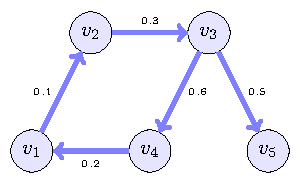
\includegraphics[width= 5cm]{simple_graph_example_for_regular_normalization.pdf}
  \caption{}
    \label{fig:simple_ex}
\end{figure}

We thus present two methods for converting the social graph into a Markov chain, which consider (among other things) the difference between the $w_{in}(\cdot)$ values.

\subsection{The Self-Loops Method}
%$p(R_1|\mathcal{A'}),p(R_2|\mathcal{A'}),p(R_3|\mathcal{A'}),p(R_4|\mathcal{A'})$ are $0.25,0.5,0.167,0.083$, respectively. 

%$[p(R_1|\mathcal{A'}),p(R_2|\mathcal{A'}),p(R_3|\mathcal{A'}),p(R_4|\mathcal{A'})] = \frac{1}{z}[0.1\cdot 0.3\cdot 0.6, 0.3\cdot 0.6\cdot 0.2, 0.6\cdot 0.2\cdot 0.1 , 0.2\cdot 0.1\cdot 0.3] =[0.25, 0.5, 0.1666, 0.08333]$


% $p(R_2|\mathcal{A'})=\frac{0.3\cdot 0.6\cdot 0.2}{0.6} = 0.6$,
% $p(R_3|\mathcal{A'})=\frac{0.6\cdot 0.2\cdot 0.1}{0.6} = 0.2$,
% $p(R_4|\mathcal{A'})=\frac{0.2\cdot 0.1\cdot 0.3}{0.6} = 0.1$.
% 


%(!! maybe to add a note, that those calculations ARE precise, since there is no subgraph that contain two different out-trees)

 


In our first approach, \textit{Self-loops}, after converting all the edges of $G_N[A']$, we add self-loops to all states. This allows us to normalize the edge probabilities by dividing all of the weights by the same number. Specifically, let $max_{in} = \max_{v_i\in A'} w_{in}(v_i)$ (We compute $w_in$ in the graph $G_N[A']$).
%let $max_{in} = \max_{v_i\in V_N}w_{in}(v_i)$. 
The self-loops methods works as follows;
\begin{enumerate}
    \item Convert each node $v_i \in G_n[A']$ into a state $s_i$ and each edge $(v_i,v_j)$ into a reversed edge $(s_j,s_i)$ with $q^{ji} = \frac{p^{ij}}{max_{in}}$.
    \item For each $s_i$, add a self loop $(s_i,s_i)$ with $q^{ii}=\frac{max_{in}-w_{in}(v_i)}{max_{in}}$
    %\item divide each of the transition probabilities by $max_{in}$. 
    \item Compute the stationary distribution $\Pi$.
    \item $\hat{\Gamma}$ is assigned the values of $\Pi$. 
    %\item Output $\arg\max_{v_i\in V_N} \hat{\Psi}_i$.
\end{enumerate}


% First add a self loop $(s_i,s_i)\in E_M$, with a weight $q^{ii}=1-\frac{w_{in}(v_i)}{max_{in}}$.
% For every 

% $s_i, s_j \in S_M$, we set $q^{ij}=\frac{p^{ji}}{max_{in}}$, and for each state $s_i \in S_M$ we add a self loop $(s_i,s_i)\in E_M$, with a weight $q^{ii}=1-\frac{w_{in}(v_i)}{max_{in}}$.




% Next, each edge $(v_i,v_j)\in E_N$ with probability $p^{ij}$, that have both its nodes in $A'$, becomes a (reversed) edge $(s_j,s_i)\in E_M$.
% In addition, for every state $s_i \in V_M$ we add a self loop $(s_i,s_i)\in E_M$.
% Let $d_{in}(v_i)=\sum_{v_j\in V_N}p^{ji}$, and let $m = \max_{v_i\in V_N}d_{in}(v_i)$.
% For every self loop $(s_i,s_i)\in E_M$ we assign a transition probability: $ q^{ii}=\frac{m-d_{in}(v_i)}{m}$, end every edge (that is not a self loop) $(s_j,s_i)\in E_M$ is assigned a transition probability $q^{ji}:=\frac{p^{ij}}{m}$.
% Observe that for every state $s_i\in V_M$, $\sum_{s_j\in V_M}q^{ij}=1$.%maybe to add this as part of the thm?

Clearly, the transition probabilities are valid. We need to show that $\hat{\Gamma}$ is restored correctly. 


\begin{theorem}
\label{SelfLoop}
(Self-loops method)

For the self-loops method, for every $1\leq i \leq |A'|$ it holds that $\Psi_i =\alpha \cdot \Gamma_i$,
where $\alpha$ is a constant.
In other words, For every node $v_i\in G_N[A']$, the sum of weights of all out-trees spanning $A'$ and rooted at $v_i$,
is proportional to the sum of weight of all in-trees in $G_M$ that span all states and are rooted at the corresponding state $s_i$. 
\end{theorem}
\begin{proof}
Observe that every spanning out-tree $T \subseteq G_N[A']$, with weight $w(T)=\prod_{e\in T}p^e$ has a corresponding spanning in-tree $T' \subseteq G_M$ with weight $w(T')$. In addition,
in-trees do not contain self loops, and have exactly $n-1$ edges (where $n=|A'|$). Therefore,
\[
 w(T')=\prod_{e\in T'}q^e = \prod_{e\in T}\frac{p^e}{max_{in}} =\frac{1}{(max_{in})^{n-1}}\cdot \prod_{e\in T}p^e 
%= \frac{1}{(max_{in})^{n-1}}\cdot w(T) 
=\alpha \cdot w(T).
\]
Thus,
\[
\Psi_i = \sum_{T'\in IT_{i,S_M}}w(T')
% \]
% \[
 = \alpha \cdot \sum_{T\in OT_{i,V_N}} w(T)=\alpha \cdot \Gamma_i.
\]
\end{proof}

Clearly, it can be concluded that $\hat{\Psi} = \hat{\Gamma}$.
Note that the stationary distribution $\Pi$ that is calculated by the self loops method, is equal to $\hat{\Psi}$ (by Theorem \ref{TreeThm}), and is also equal to $\hat{\Gamma}$. Therefore, by using the self loops method for the conversion and selecting the node $v_i$ with the maximal $\hat{\Gamma}_i$, we obtain a good estimation for $v^*$. 
%Therefore, the self loops method outputs the node with maximal $\hat{\Gamma}_i$ value, as required.
%Clearly, $\hat{\Psi}_i$ is equal to $\hat{\Gamma}_i$. 

%%%%%%%%%%%%%%%%%%%%%%%%%%%%%%%%%%%%%%%%%%%%%%%%%%%5!!!!!!


\begin{figure}[hbpt] 
    \centering
    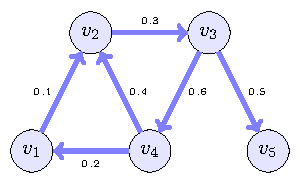
\includegraphics[width= 6cm]{example.pdf}
  \caption{}
    \label{fig:complex_ex}
\end{figure}

\begin{figure}[hbpt] 
    \centering
    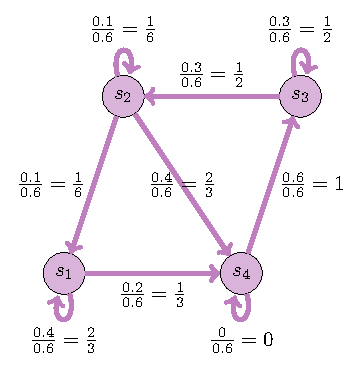
\includegraphics[width= 6cm]{self_loop_markov_chain.pdf}
  \caption{The Markov chain that corresponds to the social network of Figure \ref{fig:complex_ex} (with $max_{in}=0.6$).}
    \label{fig self loop mc}
\end{figure}

%an example for self loop
%Next we show an example that is a bit more complex. 
To demonstrate the self-loops method and Theorem \ref{SelfLoop}, we consider the social network given in Figure \ref{fig:complex_ex}, which is slightly more complex than the graph in Figure \ref{fig:simple_ex}, as it includes an additional edge between $v_4$ and $v_2$.
Now, assume that the set of active nodes is $A= \set{v_1,v_2,v_3,v_4,v_5}$.
Clearly, $A'=\set{v_1,v_2,v_3,v_4}$, 
The self-loop method computes
the Markov chain that is shown in Figure \ref{fig self loop mc},
and the stationary distribution of this Markov chain is $\Pi = (0.125,$ $0.25,$ $0.417,$ $0.208)$. Recall that $\Pi= \hat{\Psi}$, (according to Theorem~\ref{TreeThm}), and $\hat{\Psi}=\hat{\Gamma}$ (according to Theorem~\ref{SelfLoop}).
Indeed, using the out-tree counting method for directly calculating the values of $\Gamma$ leads to the same result. Specifically, $v_1$ has one possible spanning out-tree with $\Gamma_1 = 0.1\cdot 0.3 \cdot 0.6 = 0.018$. $v_2$ has one possible spanning out-tree with $\Gamma_2= 0.3\cdot 0.6\cdot 0.2=0.036$. $v_3$ has two possible spanning out-tree with $\Gamma_3 =0.6\cdot 0.2 \cdot 0.1 +0.6\cdot 0.2 \cdot 0.4=0.06$ (see Figure \ref{figv3}), and $v_4$ has two possible spanning out-tree with $\Gamma_4 =0.2\cdot 0.1 \cdot 0.3 +0.2\cdot 0.4 \cdot 0.3=0.03$ (see Figure \ref{figv4}). Therefore, $\Gamma = (0.018,$ $0.036,$ $0.06,$ $0.03)$, and $\hat{\Gamma}$ equals $\Pi$. Overall, the self-loops method outputs the vertex $v_3$ as the most likely source node.

% \begin{figure}[hbpt] 
%     \centering
%     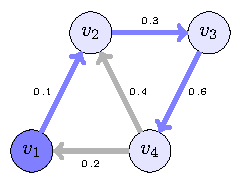
\includegraphics[width= 4cm]{example_spreading_patterns_of_v_1.pdf}
%   \caption{A spanning out-tree rooted at $v_1$.}
%     \label{figv1}
% \end{figure}


% \begin{figure}[hbpt] 
%     \centering
%     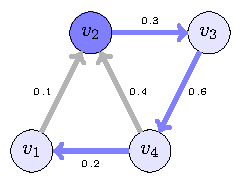
\includegraphics[width= 4cm]{example_spreading_patterns_of_v_2.pdf}
%   \caption{A spanning out-tree rooted at $v_2$}
%     \label{figv2}
% \end{figure}

\begin{figure}[hbpt] 
    \centering
    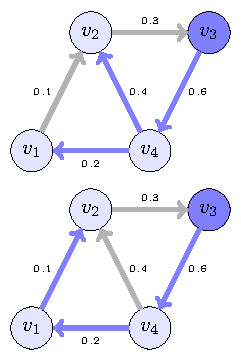
\includegraphics[width= 4cm]{example_spreading_patterns_of_v_3.pdf}
  \caption{Two spanning out-trees rooted at $v_3$.} 
    \label{figv3}
\end{figure}

\begin{figure}[hbpt] 
    \centering
    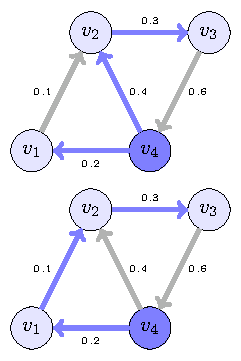
\includegraphics[width= 4cm]{example_spreading_patterns_of_v_4.pdf}
  \caption{Two spanning out-trees rooted at $v_4$.} % The corresponding weight is $0.2\cdot 0.1 \cdot 0.3 +0.2\cdot 0.4 \cdot 0.3=0.03$.}
    \label{figv4}
\end{figure}

Note that the \textit{precise} brute force calculation outputs the values $(0.1315,0.2631,$ $0.4035,$ $0.2017)$, and thus it also determines that $v_3$ is the most likely source node. Furthermore, the correlation between the exact probabilities to $\Pi$ is $0.9966$. %(the complete number is "0.99667245" )
% !! maybe we should add the full calculation as an appendix?

\begin{figure}[hbpt] 
    \centering
    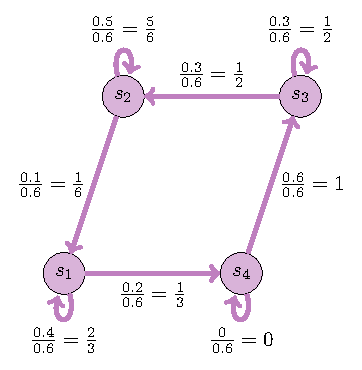
\includegraphics[width= 5cm]{self_loop_markov_chain_simple_graph.pdf}
  \caption{The Markov chain that is obtained by applying the self loops method on the graph of Figure \ref{fig:complex_ex}.}
    \label{fig simple self loops markov chain}
\end{figure}

Returning to the example in Figure \ref{fig:simple_ex}, the corresponding Markov chain that is obtained by the self loops method is shown in figure \ref{fig simple self loops markov chain}, and the stationary distribution for this Markov chain is $\Pi=(0.25,$ $ 0.5,$ $ 0.167,$ $0.083)$. 
That is, in this example the self-loops method finds the exact probabilities, since for every sub-graph of $G_N[A']$ there is at most one spanning out-tree. % (as computed in Section \ref{sec: conversion method}).


%(where should we wright the justification for the no-loops method? now, or after we describe it? (the justification is that when using random walk for calculating the stat. dist. the no-loops is faster...)
%also - we need a better name for it ...

%regular normalization with FIX method

%(this should be after the figure 7....)

\subsection{The no-loops Method}
Recall that the self-loops method returns the exact values of $\hat{\Gamma}$ when $\Pi$ is computed directly. However, when $\Pi$ is estimated by sampling, the addition of the self loops to the graph might require longer random walks, as many of the random steps are ``wasted'' on the self loops. This, in-turn, may affect the efficiency of the sampling.
Therefore, we present our second method, \textit{no-loops}, which does not add self-loops to the states. Instead, it first computes the edge probabilities using the naive method. Once the stationary distribution $\Pi$ is computed, the no-loops method restores the correct $\hat{\Gamma}$ values from $\Pi$ by dividing each $\Pi_i$ by $w_{in}(v_i)$ and normalizing the result.

% the $\Pi_i$ values for every $i$ and normalizes this. This provides a new distribution $\Pi'$. We then output $\arg \max \Pi'_i$.
% (temporal name...)) 
Specifically, the no-loops method is executed as follows:
\begin{enumerate}
    \item Convert each node $v_i \in G_n[A']$ into a state $s_i$ and each edge $(v_i,v_j)$ into a reversed edge $(s_j,s_i)$ with $q^{ji} = \frac{p^{ij}}{w_{in}(v_j)}$. %should we reverse it to ji -> ij ? (and do the same for the self loop method... (that way, we will have ${w_{in}(v_i)$ in the denominator...)
    \item Compute the corresponding stationary distribution $\Pi$.
    \item Let $\Pi^{corr.} =$ $ (\Pi^{corr.}_1,$ $ \ldots, \Pi^{corr.}_{|A'|})$, where $\Pi^{corr.}_i =$ $\frac{\Pi_i}{w_{in}(v_i)}$.
    %\item Let $\Pi' = (\Pi'_1,\Pi'_2,\ldots,\Pi'_{|A'|})$, where $\Pi'_i = \frac{\Pi_i}{w_{in}(v_i)}$.
    \item $\hat{\Gamma}$ is assigned the values of $\hat{\Pi}^{corr.}$.
    % \item $\hat{\Gamma}$ is assigned the values of $\Psi'$. 
    %\item Output $\arg\max_{v_i\in V_N} \hat{\Psi}_i$.
    
\end{enumerate}

We now show that $\hat{\Gamma}$ is restored correctly.  Indeed, the no-loops method converts the social network to a Markov chain using the naive method. We show that with this conversion, the weight of each spanning out-tree is divided by a value that depends only on the root node.
%in the Markov chain contains exactly one edge that is divided by each of the nodes in-degrees, except the root. 
Therefore, in order to restore $\hat{\Gamma}$ we must multiply each $\Pi_i$ by this value. Indeed, as we show, instead of multiplying by this value, it is sufficient to divide by $w_{in}(v_i)$.

%%%%%% until here 7/12/22


\begin{theorem}\label{NoLoop}
(No-loops method)

For the no-loops method, for every $1\leq i \leq |A'|$ it holds that $\frac{\Pi_i}{w_{in}(v_i)} =\alpha \cdot \Gamma_i$,
where $\alpha$ is a constant.

%Alternatively:, this sentence should be the first paragraph of the proof, and the theorem will be something simpler like "the outputs of both methods equal"...

\end{theorem}

\begin{proof}
%another try:
Observe that we can divide the edge set of $G_N[A']$ to $n$ sections by their end node.
When we convert the graph and normalize it by the naive way, for a section $X_i = \{(v_j,v_i)|v_j\in V_N\}$, all the edge probabilities are divided by $w_{in}(v_i)$

Let us focus our attention to %the changes to the weight of 
a single spanning out-tree $T\subseteq G_N[A']$, with root $v_r$. The weight of the corresponding in-tree $T'\in G_M$, is equal to the the weight of $T$ divided by the $w_{in}(\cdot)$ values of all the nodes, except for the root. I.e. $w(T') = \frac{w(T)}{ \prod_{v_i\in V, v_i\neq v_r} w_{in}(v_i)}$. Then, if we divide $w(T')$ by $w_{in}(v_r)$, we get 
\begin{equation}
    \frac{w(T')}{w_{in}(v_r)} = \frac{w(T)}{ \prod_{v_i\in V} w_{in}(v_i)}
\end{equation}
Note that the value $\prod_{v_i\in V} w_{in}(v_i)$ does not depend on the identity of the root $v_r$.


For example, in Figure \ref{fig: no loop in-tree out-tree}, $T$ is a spanning out-tree of a certain graph $G_N[A']$ with the root $v_1$, and $T'$ is the corresponding in-tree of the Markov chain $G_M$. The edge probabilities are detailed in the figure. $w(T) = p^{1,2} \cdot p^{1,3}\cdot p^{2,4} \cdot p^{2,5}\cdot p^{3,6}$,
and
$w(T') = \frac{w(T)}
{\prod_{i=2}^6 w_{in}(v_i)}$.
 After dividing $w(T')$ by $w_{in}(v_1)$ we get 
$
     \frac{w(T')}{w_{in}(v_1)}= \frac{w(T)}{\prod_{i=1}^6w_{in}(v_i)}
$
 
 
\begin{figure}[hbpt] 
    \centering
    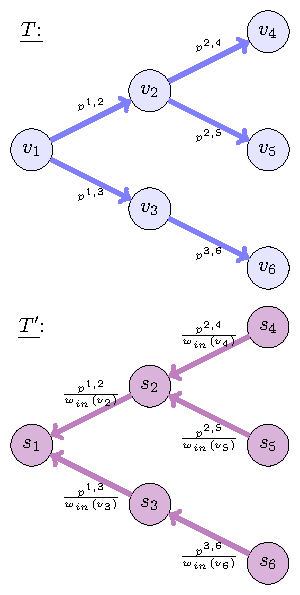
\includegraphics[width= 5cm]{no_loop_out_tree_vs__in_tree (1).pdf}
  \caption{$T$ is a spanning out-tree  of a graph $G_N[A']$ with $v_1$ as it's root, and $T'$ is the corresponding in-tree in the corresponding Markov chain.
  }

    \label{fig: no loop in-tree out-tree}
\end{figure}




%*************
Let $T$ be a spanning out-tree in $G_N[A']$, rooted at $v_r$ with weight $w(T)$. %Recall that every node in an out-tree has exactly one in-edge, except for the root node that has no in-edges.
Additionally, let $T'$ be the spanning in-tree in $G_M$ that corresponds to $T$.
Each edge $(s_j,s_i) \in T'$ has a weight $q^{ji} = \frac{p^{ij}}{w_{in}(v_i)}$. 
Therefore, the weight of $T'$ is:

\[
w(T') = \prod _{(s_j,s_i)\in T'} q^{ji}
=\prod _{(v_i,v_j)\in T} \frac{p^{ij}}{w_{in}(v_i)} 
\]
Since in the in-tree $T'$, the root node $v_r$ does not have an out-edge, the denominator is a multiplication of all the $w_{in}(v_i)$ values except for $w_{in}(v_r)$:
\[
w(T') =\frac{1}{\prod _{v_i\in V_M , i\neq r} w_{in}(v_i)} \cdot \prod _{(v_i,v_j)\in T} p^{ij}
\]
\[
=\frac{1}{\prod _{v_i\in V_M , i\neq r} w_{in}(v_i)} \cdot w(T)
\]

For $\Pi$ that is calculated in stage $(2)$ of the no-loops method, we get that for every $1\leq i\leq |A'|$ it holds that \[
\Pi_i = \sum w(T') = \frac{1}{\prod _{v_j\in V_M , j\neq i} w_{in}(v_j)} \cdot \sum_{T\in OT_{i,A'}}w(T)
\]
\[
= \frac{1}{\prod _{v_j\in V_M , j\neq i} w_{in}(v_j)} \cdot \Gamma_i
\]

Then for $\Pi^{corrected}_i$, since every $\Pi^{corrected}_i = \frac{\Pi_i}{w_{in}(v_i)}$ we get that
for every $1\leq i \leq |A'|$: 

\[
%\Psi'_i 
\Pi^{corrected}_i= \frac{1}{\prod _{v_j\in V_M } w_{in}(v_j)} \cdot \Gamma_i
= \alpha \cdot \Gamma_i
\]
($\alpha$ is a constant since the denominator does not depend on $i$). 
\end{proof}



Here We can conclude that $\arg \max \Psi' = \arg \max \Gamma$. Therefore the no-loops method also outputs the node with maximal $\Gamma_i$ value. Moreover, the output of the no-loops method equals to the output of the self-loops method.


\subsubsection{A Numerical Example}
If we go back to the example of Figure \ref{fig:complex_ex}, 
the Markov chain that the no-loops
you can find the corresponding Markov chain, by the no-loops method in Figure \ref{fig no-loops mc}.
The stationary distribution of the Markov chain of Figure \ref{fig no-loops mc} is $\Pi=(0.0625,0.3125,0.3125,0.3125)$.
The Fix method will give:
%Let $\prod _{j=1}^nd_{in}(v_j)=0.2\cdot 0.5\cdot 0.3\cdot 0.6 = 0.018$.
$\Pi'=(\frac{0.0625}{0.2},\frac{0.3125}{0.5},\frac{0.3125}{0.3},\frac{0.3125}{0.6})$ 
and after normalization we get 
$(0.125,$ $0.25,$ $0.417,$ $0.208)$
which is equal to the output we got with the previous method.


\begin{figure}[hbpt] 
    \centering
    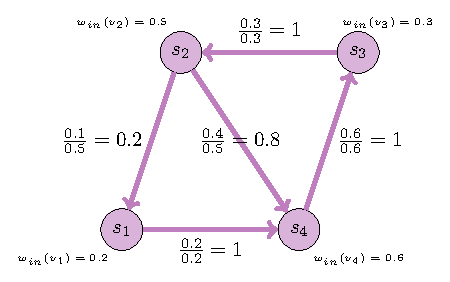
\includegraphics[width= 6cm]{no_loop_markov_chain.pdf}
  \caption{The Markov chain that corresponds to the social network of Figure \ref{fig example} by the no-loops method.
  %to change the d_{in} to a sign we agree on...
  }
    \label{fig no-loops mc}
\end{figure}

%to do 12.9:
%Amos's method
%with proofs

%an example for self loop, big mother, Amos's method and the regular with FIX.
%






% \section{The proposed algorithm SDSD}



% for the big mother alternative, we matched a different type of random walk, that is basically based on the algorithm for finding a random spanning tree in a graph. (\cite{}).


% \section{Results}

% (we also tried several other options: simple normalization, permutation based normalization)
%  in addition we ran a few heuristics to compare our algorithms results.


%****to check the algorithms on the Continuous time IC model...***** 

\section{Experiments}
% framework:
% 1. general information on the data-set and the filtering of the nodes that we did
% 2. the heuristics we show.
% 3. our results and discussion on it
%to add the computer details....

For the evaluation of the performance of the self-loops and the no-loops methods, and comparing it to other baselines heuristics, we used $14$ types of directed random graphs that have diffusion probabilities on their edges. Each graph type has the following parameters: $(n, Density, p_{range})$. We built the graphs as follows: first we initialize $n$ nodes. then each possible directed edge was inserted to the graph with a probability of $Density$. Then, for every edge $(v_i,v_j)$, we assigned to $p^{ij}$ a random number from the range $[0,p_{range}]$.

we built $1,000$ instances for each of those $14$ graph types. In Table \ref{tab:graphs} we summarized the parameters of the sampled graphs:

% the computer details: Intel i7-7500U computer (clocked at 2.9GHz with 16GB RAM). %with 4 cores (we need to add Noam's computer details..)

\begin{table}[hbpt]
  \caption{Graphs types details}
  \label{tab:graphs}
  \begin{tabular}{l c c c r}\toprule
    Graphs & n & Density &$P_{range}$ & Average number of edges \\ \midrule
    $G_1$& 500	& 0.1 & 0.0416 &	24957\\
    $G_2$& 1000 & 0.1 & 0.0204 & 99,909\\
    $G_3$& 2000	& 0.1 & 0.0101 & 399,785\\
    $G_4$& 3000	& 0.1 & 0.0071 &	899,721\\
    $G_5$& 4000 & 0.1 & 0.0052 &	1,599,576\\
    $G_6$& 5000 & 0.1 & 0.0041 & 2,499,461\\
    \midrule
    $G_7$&  500  &	0.0416 &	0.1 &	10,404\\
    $G_8$&  1000 &	0.02 &	    0.1	&   20,022\\
    $G_9$&  2000 &	0.0101 &	0.1	&    40,394\\
    $G_{10}$&3000 &	0.0067 &	0.1	&   60,392\\
    $G_{11}$&4000 &	0.0052 &	0.1	&   84,185\\
    $G_{12}$&5000 &	0.0041 &	0.1	&   104,138\\
    $G_{13}$&10000 &	0.002 &	0.1	&   204,092\\
    $G_{14}$&15000 &	0.0013 & 0.1 &	304,001\\

    
    \bottomrule
  \end{tabular}
\end{table}

For each of the we graphs we sampled, we selected a random source node, and ran a simulation of a diffusion according to the IC model, obtaining an active set $A$.
We ignored diffusions in which the size of the active set was less that 20 nodes, and diffusions in which the size of the set  $A'$ was 1. The number of times we ignored a sampled graph is summarised in Table \ref{tab:diffusions} 

We sampled graphs until we obtained $1000$ graph instances for each of the $14$ graph types.
We summarised in \ref{tab:diffusions} the average sizes of the set $A'$ and the average amount of edges in the sub-graph induces by $A'$.

\begin{table}[hbpt]
  \caption{Diffusion details}
  \label{tab:diffusions}
  \begin{tabular}{c c c c c}\toprule
    Graph & Average & Average & no. times  & no. too small \\ 
    type &  $|A'|$ & $e(G[A'])$& $|A|=1$ & diffusions.  \\ \midrule
    $G_1$   &71.162  & 728.594 & 33 & 4,058\\
    $G_2$ 	&93.907  & 1438.516 & 21 &	4,527\\
    $G_3$	&119.167 & 2675.412 & 21 &	4,467 \\
    $G_4$   &263.945 & 12418.689 & 13 &	3,280\\
    $G_5$   &257.102 & 13200.164 & 24 &	3,305 \\
    $G_6$ 	&265.526 & 15136.812 & 20 & 3,736\\
    \midrule
    $G_7$ & 77.595 &	410.53	& 154	&4,440 \\
    $G_8$ & 92.328 &	376.151	& 469   &6,800 \\
    $G_9$ & 148.714&    550.316 & 804	&7,589 \\
    $G_{10}$ & 174.998 &	608.171	 & 1,139	 & 9,284 \\
    $G_{11}$ & 371.221 &	1504.982 &	860	 & 6,616 \\
    $G_{12}$ & 386.578 &	1460.45	& 1,073	& 7,630 \\
    $G_{13}$ & 536.922 &	1718.632&	2,163&	12,667\\
    $G_{14}$ &  607.511	& 1783.66 &	3,026	& 17,039 \\
    \bottomrule
  \end{tabular}
\end{table}

In addition to the self-loops and the no-loops methods, we also ran the following baseline heuristics. For all those heuristics, we calculate a grade for each node and output the node with the maximum grade. The heuristics differ by the way to calculate the node grades.
\begin{itemize}
    \item \textbf{Self-loops with random walk:} We build the Markov chain as in the self-loops method. In order to estimate the stationary distribution, we ran $4$ random walk simulations of $50/100/500/1000$ steps, the grade of each node $v_i$ is the percentage of steps to $v_i$ from the total amount of steps. 
    \item \textbf{no-loops with random walk:} We build the Markov chain as in the no-loops method (the naive normalisation). Estimate the stationary distribution, by $4$ random walk simulations of $50/100/500/1000$ steps, and fixed the given grades by dividing each grade by $w_{in}(v_i)$ as described in the no-loops method. 
    \item \textbf{Naive:} We build a Markov chain, where the normalization of the edges is by the naive way. The stationary distribution is used for the estimation grades, without any fixing.
    \item \textbf{Random:} a random selection of a node in $A'$. (basically, every node is assigned the grade $\frac{1}{|A'|}$).
    \item \textbf{Max out-degree:} For each node, the grade is the summation of the transition probabilities of all it's out-edges.
    \item \textbf{Min in-degree:} For each node, the summation of the transition probabilities of it's in-edges, multiplied by $-1$ is used as the node's grade.
    \item \textbf{Max (out/in) degree:} For each node, we calculate the summation of the transition probabilities of it's out edges and divide it by the summation of the transition probabilities of it's in-edges.
    \item \textbf{IM based:} For each node, we make $1000$ samples of IC model diffusions, and the average size of active set is assigned as the grade of that node.
\end{itemize}

Our results are presented in Figures \ref{tab:results}

\begin{table*}[hbpt]
  \caption{Algorithms Results}
  \label{tab:results}
  \begin{tabular}{c | c c c c c c | c c c c c c c c | r}\toprule
	&	\textbf{$G_1$}	&	\textbf{$G_2$}	&	\textbf{$G_3$}	&	\textbf{$G_4$}	&	\textbf{$G_5$}	&	\textbf{$G_6$}	&	\textbf{$G_7$}	&	\textbf{$G_8$}	&	\textbf{$G_9$}	&	\textbf{$G_{10}$}	&	\textbf{$G_{11}$}	&	\textbf{$G_{12}$}	&	\textbf{$G_{13}$}	&	\textbf{$G_{14}$}	&	\textbf{Average}	\\
	\midrule
\textbf{Self-Loops}	&	\textbf{90}	&	\textbf{80}	&	\textbf{78}	&	\textbf{50}	&	\textbf{57}	&	\textbf{73}	&	\textbf{111}	&	\textbf{137}	&	\textbf{135}	&	\textbf{156}	&	\textbf{90}	&	\textbf{115}	&	\textbf{101}	&	\textbf{115}	&	\textbf{99.14}	\\
sl rw 50	&	40	&	36	&	43	&	33	&	23	&	46	&	68	&	104	&	85	&	94	&	45	&	70	&	54	&	62	&	57.35	\\
sl rw 100	&	64	&	54	&	62	&	39	&	46	&	43	&	80	&	103	&	91	&	127	&	57	&	77	&	64	&	68	&	69.64	\\
sl rw 500	&	81	&	58	&	72	&	42	&	60	&	53	&	102	&	126	&	126	&	144	&	70	&	98	&	83	&	83	&	85.57	\\
sl rw 1000	&	79	&	74	&	65	&	49	&	54	&	58	&	105	&	136	&	109	&	141	&	75	&	98	&	84	&	100	&	87.64	\\
\midrule
 \textbf{No-Loops} 	&	\textbf{90}	&	\textbf{80}	&	\textbf{78}	&	\textbf{50}	&	\textbf{57}	&	\textbf{73}	&	\textbf{111}	&	\textbf{137}	&	\textbf{135}	&	\textbf{156}	&	\textbf{90}	&	\textbf{115}	&	\textbf{101}	&	\textbf{115}	&	\textbf{99.14}	\\
nl rw 50	&	69	&	67	&	69	&	52	&	45	&	59	&	99	&	132	&	118	&	130	&	73	&	95	&	85	&	90	&	84.5	\\
nl rw 100	&	87	&	67	&	83	&	44	&	51	&	53	&	97	&	133	&	125	&	145	&	77	&	99	&	92	&	88	&	88.64	\\
nl rw 500	&	84	&	77	&	72	&	51	&	55	&	70	&	100	&	146	&	132	&	154	&	91	&	110	&	104	&	108	&	96.71	\\
nl rw 1000	&	92	&	75	&	75	&	53	&	56	&	72	&	105	&	138	&	132	&	160	&	88	&	109	&	106	&	110	&	97.92	\\
\midrule
 \textbf{naive(simple)}	&	37	&	44	&	30	&	30	&	20	&	23	&	51	&	49	&	45	&	59	&	28	&	32	&	39	&	30	&	36.92	\\
 \textbf{random}	&	17	&	20	&	21	&	10	&	13	&	19	&	19	&	32	&	32	&	37	&	26	&	29	&	24	&	29	&	23.42	\\
 \textbf{maxout deg}	&	37	&	42	&	30	&	22	&	23	&	21	&	40	&	62	&	60	&	58	&	31	&	18	&	27	&	37	&	36.28	\\
 \textbf{minin deg}	&	52	&	39	&	52	&	22	&	33	&	40	&	54	&	44	&	39	&	38	&	27	&	22	&	26	&	32	&	37.14	\\
 \textbf{out over in deg}	&	49	&	50	&	60	&	30	&	40	&	53	&	55	&	76	&	68	&	63	&	38	&	26	&	34	&	46	&	49.14	\\
 \textbf{IM}	&	40	&	40	&	36	&	22	&	28	&	28	&	45	&	66	&	59	&	54	&	34	&	42	&	30	&	40	&	40.28	\\
    \bottomrule
  \end{tabular}
\end{table*}



%POINTS FOR DISCUSSION:

% the output of no-loops and Self LOOP are the same
% the random walk evaluations almost always are equal to the direct calculations.

%we are better then the MCMC algo, both in the aspect of time consumption and the efficiency 
















%%% The following command should be issued somewhere in the first column 
%%% of the final page of your paper.
\balance



%%%%%%%%%%%%%%%%%%%%%%%%%%%%%%%%%%%%%%%%%%%%%%%%%%%%%%%%%%%%%%%%%%%%%%%%

% % \section{Citations and References}
  

% %%%%%%%%%%%%%%%%%%%%%%%%%%%%%%%%%%%%%%%%%%%%%%%%%%%%%%%%%%%%%%%%%%%%%%%%

% %%% The acknowledgments section is defined using the "acks" environment
% %%% (rather than an unnumbered section). The use of this environment 
% %%% ensures the proper identification of the section in the article 
% %%% metadata as well as the consistent spelling of the heading.

% \begin{acks}
% If you wish to include any acknowledgments in your paper (e.g., to 
% people or funding agencies), please do so using the `\texttt{acks}' 
% environment. Note that the text of your acknowledgments will be omitted
% if you compile your document with the `\texttt{anonymous}' option.
% \end{acks}

%%%%%%%%%%%%%%%%%%%%%%%%%%%%%%%%%%%%%%%%%%%%%%%%%%%%%%%%%%%%%%%%%%%%%%%%

%%% The next two lines define, first, the bibliography style to be 
%%% applied, and, second, the bibliography file to be used.

\bibliographystyle{ACM-Reference-Format} 
\bibliography{sample}

%%%%%%%%%%%%%%%%%%%%%%%%%%%%%%%%%%%%%%%%%%%%%%%%%%%%%%%%%%%%%%%%%%%%%%%%

\end{document}

%%%%%%%%%%%%%%%%%%%%%%%%%%%%%%%%%%%%%%%%%%%%%%%%%%%%%%%%%%%%%%%%%%%%%%%%

